\chapter{Policy Iteration}\label{chapt:policy_iteration}

    In an \ac{MDP}, a common way to solve for a policy by iteratively updating the value function presented in Section
    \ref{sec:policy_iteration_preliminaries}. If the policy of \agent{2} was known, then iteratively solving the Bellman
    equation \cite{something} will converge to a policy that takes an optimal action at each state. This is known as
    \textit{Value Iteration}:
    \begin{equation}\label{eq:bellman_true}
        \begin{aligned}
                \optimal{V}(s) &= \max_{a_1}\left[R(s,a_1) +
                    \gamma\sum_{s'}\sum_{a_2\in A}T(s'|s,(a_1,a_2))\policy{2}(a_2|s) V^*(s')\right],\ \text{and}\\
                \optimal{\policy{1}}(s) &= \argmax_{a_1}\left[R(s,a_1) +
                    \gamma\sum_{s'}\sum_{a_2\in A}T(s'|s,(a_1,a_2))\policy{2}(a_2|s)V^*(s')\right].
        \end{aligned}
    \end{equation}

\section{Asymptotic Discount Optimal Policies}\label{sec:ADO_policy}

    In Chapter 2.5 of \cite{hernandez2012adaptive}, Hern\'andez-Lerma shows that an \textit{adaptive}  \ac{MDP} will
    converge to the optimal value function if the parameter estimate converges to the true parameter as inference
    iteration $b\rightarrow \infty$. Remember Assumption \ref{assump:opt_policy_err}; the true \policy{2} can be
    sufficiently represented with an optimal parameter.  The author formally proves that if $\estimate{\paramVec}^{(b)}
    \rightarrow \optimal{\paramVec}$ as $b \rightarrow \infty$, then $V(s;\estimate{\paramVec}^{(b)}) \rightarrow
    \optimal{V}(s;\optimal{\paramVec})$.  We'll rely on the mini-batch inference algorithm presented in the Chapter
    \ref{chapt:proactive_inference} to ensure that the estimate of the parameter vector converges to the optimal
    parameter.

    Whenever \agent{1} can processes a new dataset $D$ to form a new \estimate{\paramVec}, its policy can be updated by
    performing value iteration on
    \begin{equation}\label{eq:bellman_estim}
        \begin{aligned}
            V(s;\estimate{\paramVec})
                &= \max_{a_1}\left[R(s,a_1) + \gamma\sum_{s'}\sum_{a_2\in A}T(s'|s,(a_1,a_2))
                    \estimate{\policy{}}_{2}(a_2|s;\estimate{\paramVec}) V(s')\right],\ \text{and}\\
            \policy{1}(s; \estimate{\paramVec})
                &= \argmax_{a_1}\left[R(s,a_1) + \gamma\sum_{s'}\sum_{a_2\in A}T(s'|s,(a_1,a_2))
                    \estimate{\policy{}}_{2}(a_2|s;\estimate{\paramVec})V(s')\right].
        \end{aligned}
    \end{equation}


\section{Policies from Expectation Maximization}\label{sec:EM}

    While value iteration is guaranteed to converge to an optimal policy, it is not a fast algorithm, especially if it
    needs to be re-run after every new dataset $D$ is gathered. Toussaint and Storkey showed in
    \cite{toussaint2010expectation} that \ac{EM} can be used to approximate the MDP as a mixture of finite-time MDPs, as
    shown in Fig. \ref{fig:mixMDP}.

    \begin{figure}
        \centering
        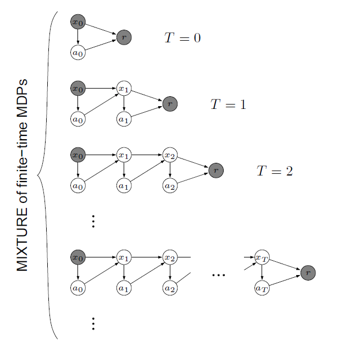
\includegraphics[width=0.6\linewidth]{mixMDP}
        \caption{Mixture of finite-time MDPs. Note this report uses notation that each finite-time MDP ends at time
                 $\Tau$.}
        \label{fig:mixMDP}
    \end{figure}

    \todo[inline]{Unsure if I can actually use this image since it's from Toussaints book. Might need to create a copy
                  of this in PowerPoint?}

    Their derivation starts with the joint distribution of the probability of a reward $\mathcal{R}$, a sequence of
    states $\traj$, and the probability of the sequence ending at time \Tau, subject to a policy $\policy{1}$. Note that
    $s^{(\Tau)}$ is the state at time \Tau in the joint distribution,
    \begin{equation} \label{eq:em_joint_dist}
        \begin{split}
            P(R,\traj,\Tau;\policy{1})
                & = P(R|\traj;\policy{1})P(\traj|\Tau;\policy{1})P(\Tau) \\
                & = P(R|s^{(\Tau)};\policy{1})\left[\prod_{t=0}^{\Tau-1}P(s^{(t+1)}|s^{(t)};\policy{1})\right]
                        P(s^{(0)};\policy{1})\delta_{|\tau|\Tau}P(\Tau),
        \end{split}
    \end{equation}
    where $\delta_{|\tau|\Tau}=1$ when the trajectory ends at step \Tau and is zero otherwise. The algorithm requires
    that each MDP in the mixture only emits a reward at a single final time step; the final states, $r$, in Fig.
    \ref{fig:mixMDP} emit rewards from the distribution $\mathcal{R}(s^{(\Tau)},a_1^{(\Tau)})$ which is defined:
    \[
    P(\mathcal{R}|s,a_t) = \frac{R(a_1,s) - \min_{a_1,s}(R)}{\max_{a_1,s}(R) - \min_{a_1,s}(R)}.
    \]

    \par
    The goal of EM is to maximize the following energy function,
    \[
    F(\policy{1},\omega) := \log P(\mathcal{R};\policy{1}) - KL(\omega(\tau,\Tau)||P(\tau,\Tau|\mathcal{R};\policy{1}).
    \]
    $F(\policy{1},\omega)$ is the difference between the log-likelihood of the reward probability subject to \policy{1},
    and the \ac{KLD} of the latent variable distribution $\omega$ from the latent variables given a reward and subject
    to $\policy{1}$. The latent, unknown, variables of the \ac{MDP} are the state-action sequence that brings the system
    to a final state, $s^{(\Tau)}$, at time $\Tau$. Note that only sequences where $|\traj|= \Tau$ provide a non-zero
    probability of reward.

    \todo[inline]{Cite some other common uses of EM.}

    \par
    The M-step returns the energy function maximized over the latent variables using the previous, texit{old},
    iteration's policy:
    \begin{equation} \label{M_step}
        \begin{split}
            F(\policy{1},\omega^*)
                & = \sum_s \left[ P(\mathcal{R}|s^{(T)};\policy{1}^{old})\alpha(s)\right]
                        \log P(\mathcal{R}|s^{(T)};\policy{1}^{old}) \\
                &\quad\ \ + \sum_{s',s}\left[ \beta(s')P(s'|s;\policy{1}^{old})\alpha(s)\right]
                        \log P(s^{(t+1)}|s^{(t)};\policy{1}^{old}),
        \end{split}
    \end{equation}
    where
    \begin{align*}
        \alpha(s^{(t)}) & = \sum_{t=0}^\infty P(s^{(t)}; \policy{1}^{old})P(\Tau=t) \text{, and}\\
        \beta(s^{(t+1)}) & = \frac{1}{1-\gamma} \sum_{\upsilon=0}^{\infty}
            P(R|s^{(t)\prime},\Tau=t+\upsilon;\policy{1}^{old})P(\Tau=\upsilon+1).
    \end{align*}
    \noindent
    In the equation for $\beta$, above, the term $s^{(t)\prime}$ refers to reachable states from $s^{(t)}$.

    Essentially, the M-step provides a policy update. The E-step, given a policy, finds the state-action sequence that
    maximizes the expectation of a reward; the E-step calculates $\alpha$ and $\beta$. These two terms are then used in
    the M-step to provide the policy for future iterations, up to $Z$ iterations. The terms $\alpha$ and $\beta$ are
    updated on a state-action horizon time-limit of $H$.  Toussaint et al. in \cite{toussaint2010expectation} show that
    as $Z\rightarrow{}\infty$, and $H\rightarrow{}\infty$, the EM algorithm returns a policy equivalent to that from VI.

    \todo[inline]{Add example.}
